\section{Architecture}
\label{section:architecture}


\begin{figure}[!h]
	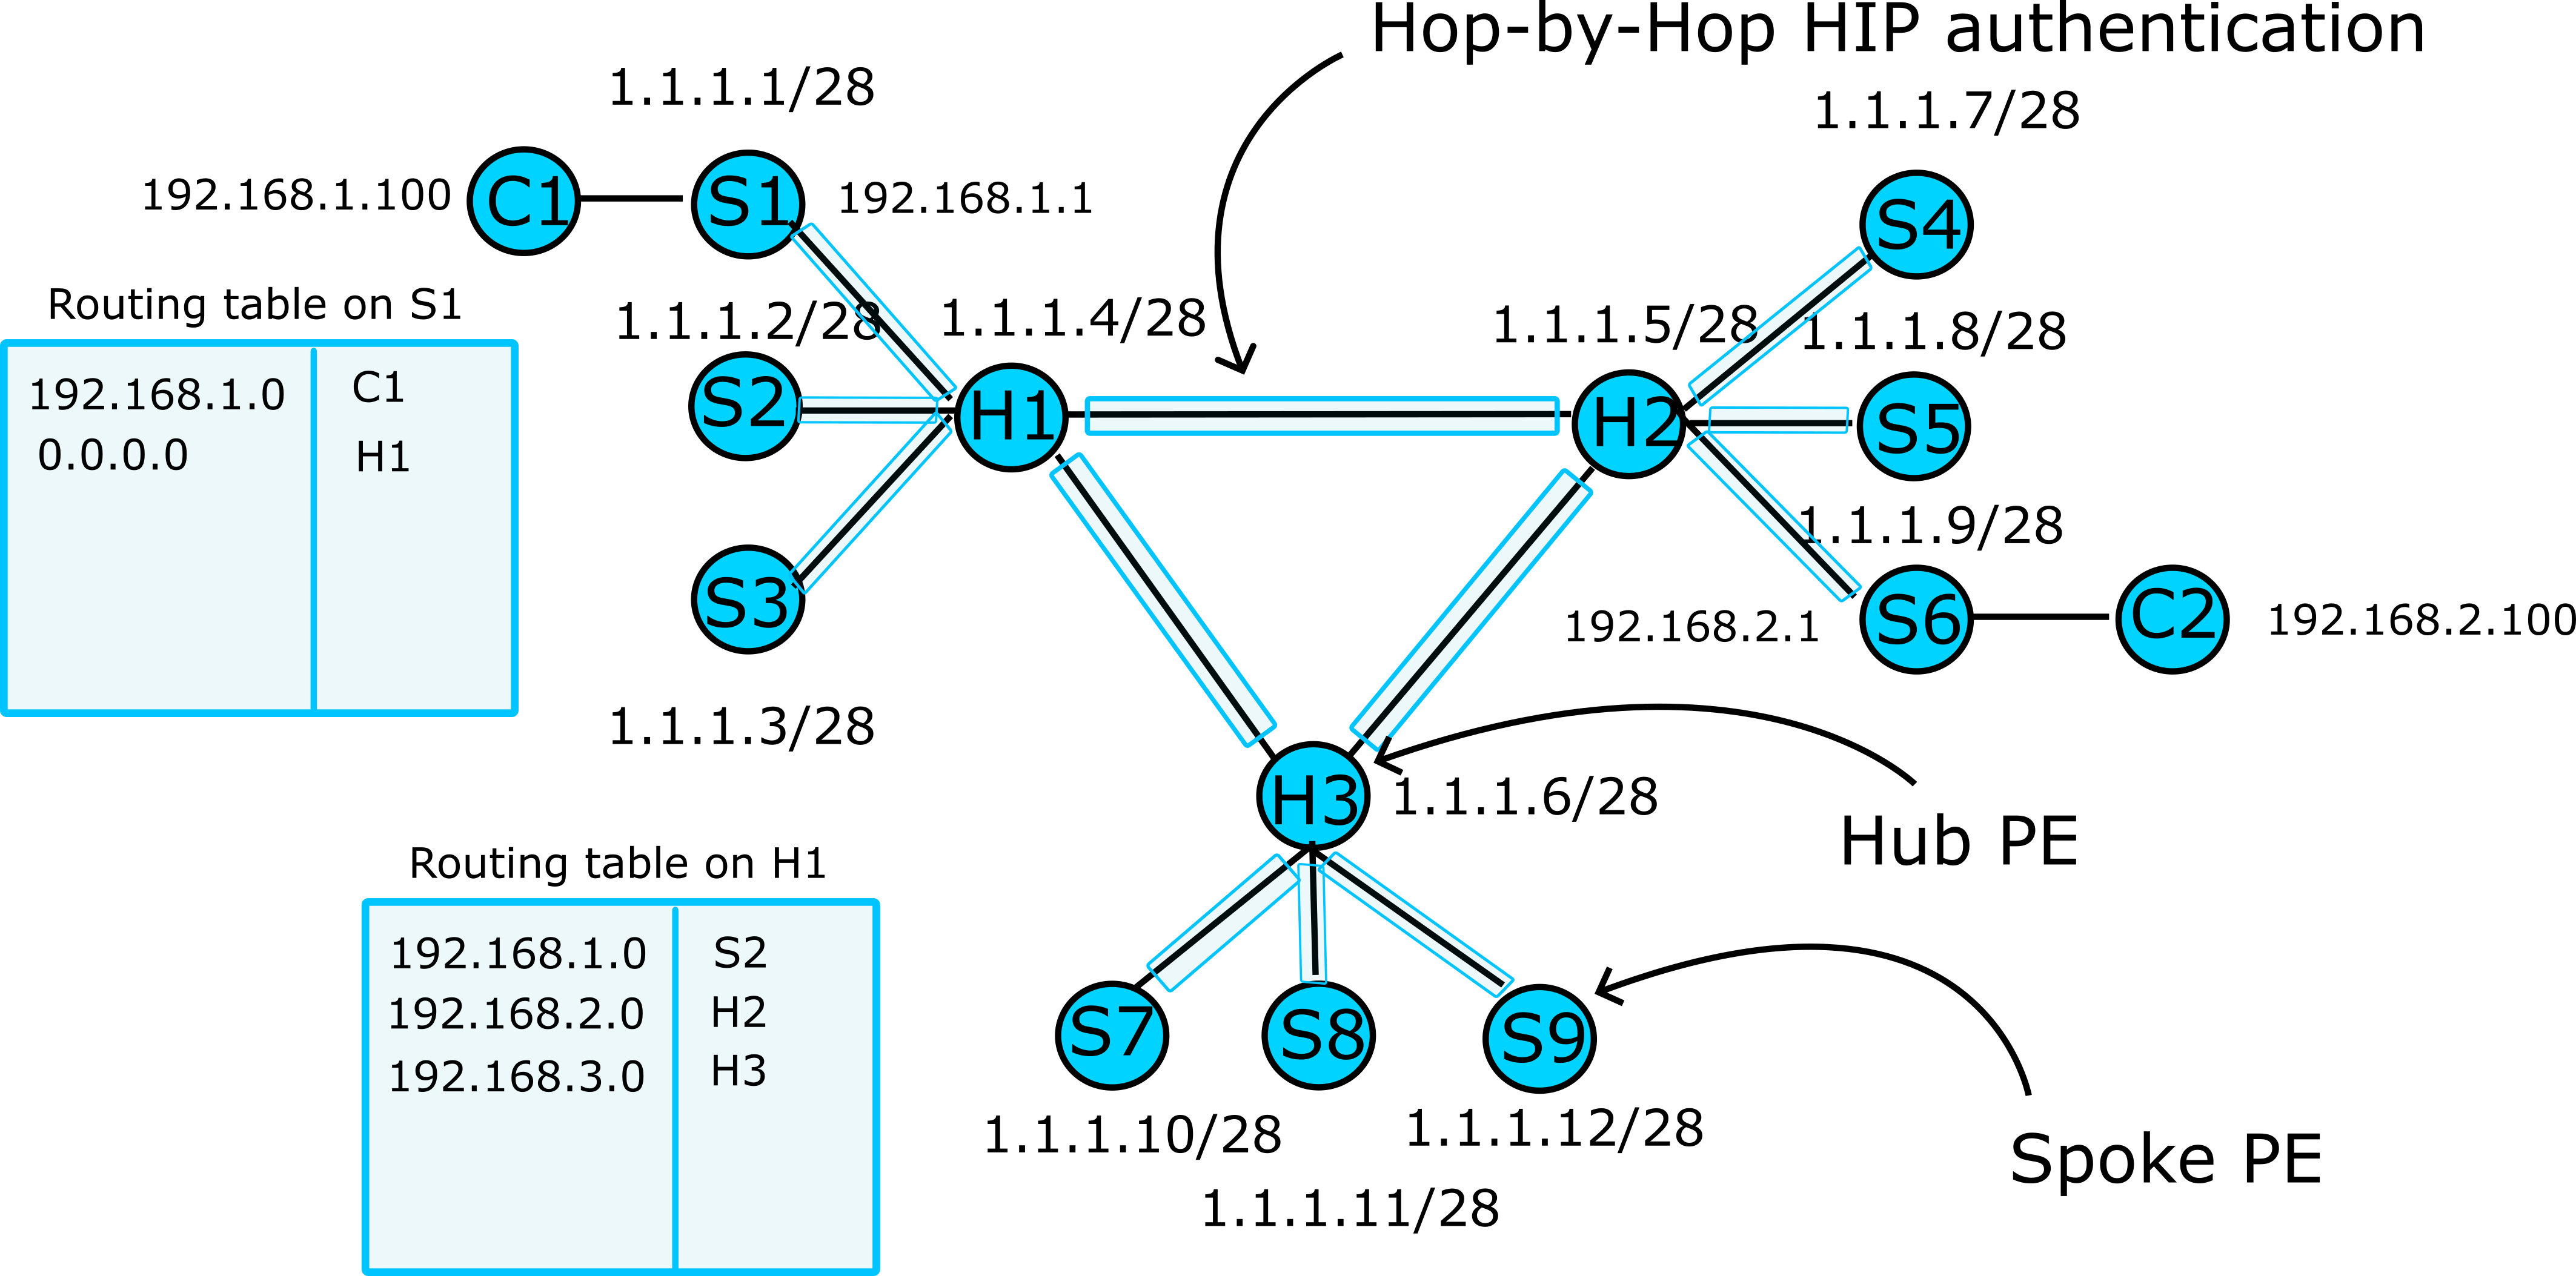
\includegraphics[width=0.5\textwidth]{graphics/arch.png}
	\caption{High-level architecture of L3-VPN deployed in Mininet}
	\label{fig:arch}
\end{figure}

\begin{table*}
        \begin{tabular}{|l|c|c|c|}
        \hline
        Characteristic $\downarrow$ \ Overlay type $\rightarrow$ & L2-VPLS & L3-VPN & HIP-VPLS \\\hline
        Size of forwarding/routing table & $O(n)$, $n$-number of hosts & $O(m)$, $m$ - number of subnetworks & $O(n)$\\\hline
        Number of links in mesh & $O(k^2)$, $k$ - number of Hub-PEs & $O(k^2)$ & $O(l^2)$, $l$ - number of PEs \\\hline
        Privacy & MACs are exposed to PEs & IPs are exposed to PEs & No exposure of MACs and IPs (PEs are part of customers inftrastructure) \\\hline
        Encryption and authentication & Hop-by-hop & Hop-by-hop & End-to-end \\\hline
        Tunneling mode & Ethernet-in-IP & IP-in-IP & Ethernet-in-IP \\\hline
        \end{tabular}
        \label{tab:analysis}
\end{table*}


The source code of the prototype is available in Github repository \url{https://github.com/dmitriykuptsov/vpls-routing}

~\cite{radiusmysql}
